\section{Définition de l'écran}

Nous définissons notre écran comme la formation d'une grille carré de pixels, la grille est de largeur $w$ (width) et de hauteur $h$ (height) en nombre de pixels. Chaque pixel a un centre qui intersecte la direction de chacun des rayons sortant de la caméra. Le centre de l'écran est le point $\mathbf{C} \in \mathbb{R}^3$ résultant de $\mathbf{E}+\vec{d}$, il se trouve ainsi à distance $1$ de la caméra. Nous définissons finalement un angle $\theta \in [-\pi,\pi]$ représetant la "Field Of View" (FOV).

Notons ici que l'écran forme un plan parrallèle à $(\vec{r},\vec{u})$ et qu'il dépend donc de l'orientation de la caméra.

Posons par exemple un écran formé par $7\times5$ pixels. La représentation finale dans $\mathbb{R}^3$ pour un FOV $\theta=\dfrac{\pi}{3}$ d'un tel écran est :

\screenrepresentation

\subsection{Aspect Ratio}
Or nous nous rendons compte que le nombre de pixels en width et en height ne sont pas toujours égaux, donc pour un même FOV nous obtenons un effet d'étirement de l'image. C'est pourquoi nous introduisons l'Aspect Ratio :

Nous pouvons visualiser un écran à  $(w,h)=(4,2)$ avant la prise en compte de l'aspect ratio :

\stretched

Les pixels ne sont pas carrés et lorsque nous représentont des objets sur ce type d'écran, nous voyons l'effet suivant :

\begin{figure}[H]
\centering
\begin{minipage}{.5\textwidth}
  \centering
  
\includegraphics[scale=0.2]{include/exemple480x480.png}
  \captionof{figure}{480x480 image}
  \label{fig:test1}
\end{minipage}%
\begin{minipage}{.5\textwidth}
  \centering
  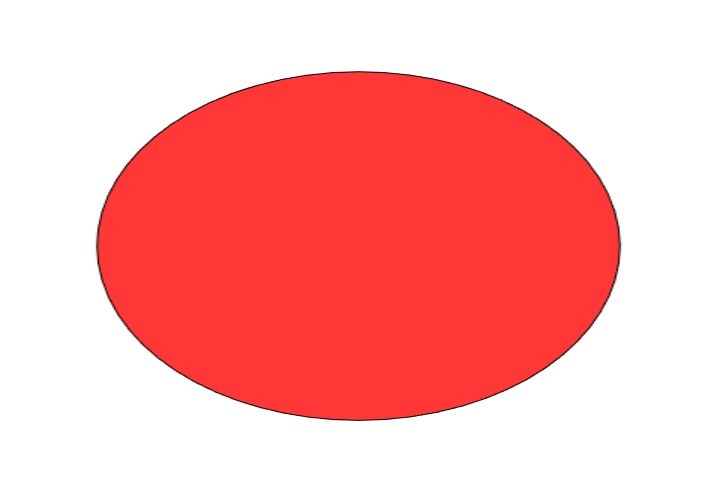
\includegraphics[scale=0.2]{include/exemple720x480.jpeg}
  \captionof{figure}{720x480 image}
  \label{fig:test2}
\end{minipage}
\begin{minipage}{.5\textwidth}
  \centering
  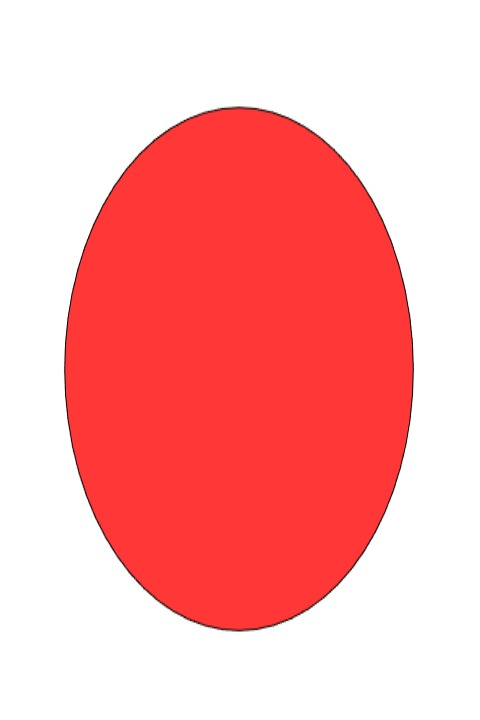
\includegraphics[scale=0.2]{include/exemple480x720.jpeg}
  \captionof{figure}{480x720 image}
  \label{fig:test3}
\end{minipage}
\end{figure}

L'aspect ratio se résume au quotient entre la width et la height de l'image en nombre de pixels : $AR=\dfrac{w}{h}$. Pour les figures ci-dessus : 

\begin{itemize}
    \item $AspectRatio_1 = \frac{480}{480} = 1$. \vspace{3pt}
    \item $AspectRatio_2 = \frac{720}{480} = 1.5 > 1$. \vspace{3pt}
    \item $AspectRatio_3 = \frac{480}{720} = 0.66 < 1$. \vspace{3pt}
\end{itemize}

Afin de corriger ce problème, nous multiplions la width $w$ par l'aspect ratio. Ainsi si $(w,h)=(4,2)$ :

$AspectRatio = \frac{4}{2} = 2$ \vspace{3pt}

\unstretched

\subsection{Obtention des vecteurs des rayons}
Nous voulons dans cette partie déterminer comment obtenir chacun des vecteurs dirigeant les rayons en fonction du nombre des pixels $(w,h)$ et de l'angle $\theta$.

Nous posons $\forall (i,j) \in \mathbb{N} \text{ tel que } 1\leq i\leq w, 1\leq j\leq h \; P_{i,j} \in \mathbb{R}^3$ chacun des centres des pixels tels que pour $(w,h)=(7,5)$ :

\begin{tikzpicture}
    \Grilleblank
    \node[above] at (0.5,6.41) {$P_{1,1}$};
    \node[above] at (4.5,6.41) {$P_{w,1}$};
    \node[below] at (0.5,0.59) {$P_{1,h}$};
    \node[below] at (4.5,0.59) {$P_{w,h}$};
\end{tikzpicture}

Par simples règles de trigonométrie sur des triangles rectangles, nous savons que :

\triangles

Remarquons que le résultat de cette distance sur la width est $\dfrac{w}{h}tan(\dfrac{\theta}{2})$, il suffit de multiplier par l'aspect ratio.

Nous pouvons maintenant chercher la distance séparant deux centres de pixels adjacents, c'est-à-dire la distance :

\distanceq et trouvons qu'elle est égale à $\dfrac{2\, tan(\dfrac{\theta}{2})}{w}$.

Nous savons que $\mathbf{C}=\mathbf{E}+\vec{d}=(0,0,1)$ et cherchons à déterminer les coordonnées de $P_{1,1}$ :

Avant cela, nous devons nous assurer de la position de $\mathbf{C}$ par rapport au centre des pixels sur l'écran. Celle-ci dépend de la paritée de $(w,h)$ donnant quatre cas de figure :

\paritee

Dans chacun de ces cas, nous pouvons tout de même obtenir les coordonnées de $P_{1,1}$ car aux vecteurs suivants : \\[0.5ex]
$\vec{d_{r}} = -2\, (\dfrac{w}{h})\, tan(\dfrac{\theta}{2}) \, \dfrac{w-1}{2w}\, \vec{r}$ \: et \: $\vec{d_{u}} = 2\, tan(\dfrac{\theta}{2}) \, \dfrac{h-1}{2h}\, \vec{u}$ \\[0.6ex]
Qui, partant de $\mathbf{C}$, pour $(w,h)=(5,7)$ sont visuellement représentées tels que : \\[0.6ex]
\begin{tikzpicture}
    \Grilleblank
    \node[above] at (0.5,6.41) {$P_{1,1}$};
    \draw[->, very thick, red] (2.5, 3.5) -- (0.5,3.5) node[below, midway, fill=white, fill opacity=0.5, text opacity=1, rounded corners] {$\vec{d_{r}}$};
    \draw[->, very thick, red] (2.5, 3.5) -- (2.5,6.5) node[right, midway, fill=white, fill opacity=0.5, text opacity=1, rounded corners] {$\vec{d_{u}}$};
\end{tikzpicture}

Nous en déduisons que les coordonnées de $P_{1,1}$ sont donc :

$P_{1,1}
=\vec{d_{r}}+\vec{d_{u}}+\mathbf{C}
=-tan(\dfrac{\theta}{2}) \, \dfrac{w-1}{h}\, \vec{r}+tan(\dfrac{\theta}{2}) \, \dfrac{h-1}{h}\, \vec{u}+\mathbf{C}$ \\[0.6ex]
$P_{1,1}
=\begin{pmatrix} -tan(\dfrac{\theta}{2}) \, \dfrac{w-1}{h}\\[1ex] 0\\0 \end{pmatrix}+\begin{pmatrix} 0\\ tan(\dfrac{\theta}{2}) \, \dfrac{h-1}{h}\\[1ex] 0 \end{pmatrix}+\begin{pmatrix} 0\\0\\1 \end{pmatrix}$ \\[0.6ex]
$P_{1,1}=\begin{pmatrix} -tan(\dfrac{\theta}{2}) \, \dfrac{w-1}{h}\\[1.3ex] tan(\dfrac{\theta}{2}) \, \dfrac{h-1}{h}\\[1.3ex] 1 \end{pmatrix}$.

De cette manière, nous pouvons finalement exprimer $P_{i,j}$ en fonction de $(w,h), \theta$ et $P_{1,1}$ :

$P_{i,j}=P_{1,1}+(i-1)\dfrac{2}{w}tan(\dfrac{\theta}{2})\vec{r}-(j-1)\dfrac{2}{h}tan(\dfrac{\theta}{2})\vec{u}$ \\[1.5ex]
$P_{i,j}=\begin{pmatrix} -tan(\dfrac{\theta}{2}) \, \dfrac{w-1}{h}\\[1.3ex] tan(\dfrac{\theta}{2}) \, \dfrac{h-1}{h}\\[1.3ex] 1 \end{pmatrix} + \begin{pmatrix} (i-1)\dfrac{2}{w}tan(\dfrac{\theta}{2})\vec{r}\\[1.3ex]0\\0 \end{pmatrix} + \begin{pmatrix} 0\\-(j-1)\dfrac{2}{h}tan(\dfrac{\theta}{2})\vec{u}\\[1.3ex]0 \end{pmatrix}$ \\[1.5ex]
$P_{i,j}=\begin{pmatrix} (i-1)\dfrac{2}{w}tan(\dfrac{\theta}{2})-tan(\dfrac{\theta}{2}) \, \dfrac{w-1}{h}\\[1.3ex] -(j-1)\dfrac{2}{h}tan(\dfrac{\theta}{2})+tan(\dfrac{\theta}{2}) \, \dfrac{h-1}{h}\\[1.3ex]1 \end{pmatrix}$ \\[2ex]
Et donc les vecteurs directeurs de chacun de ces points partant de la caméra sont :

$\forall (i,j) \in \mathbb{N} \text{ tel que } 1\leq i\leq w, 1\leq j\leq h, \; \vec{p_{i,j}} \in \mathbb{R}^3, \; \vec{p_{i,j}}=\overrightarrow{\mathbf{E}P_{i,j}}$ qui en particulier coïncide avec les coordonnées de $P_{i,j}$.

Nous voulons cependant normaliser ces vecteurs, nous définissons donc :

$\forall (i,j) \in \mathbb{N} \text{ tel que } 1\leq i\leq w, 1\leq j\leq h, \; \vec{r_{i,j}} \in \mathbb{R}^3, \; \vec{r_{i,j}}=\dfrac{\vec{p_{i,j}}}{\lVert \vec{p_{i,j}} \rVert}$. Les $\vec{r_{i,j}}$ sont les rayons normalisés sortant de la caméra dont nous connaissons maintenant les coordonnées.